% \title{Apunte de Matemáticas Discretas CC3101:\\ 
%   Introducción a Árboles Clase 22}
% % \title{Ejercicios Lógica e Inducción}
% \author{Andrés Abeliuk}
% \date{}
% \maketitle

\section{Árboles}

\subsection{Motivación e historia}

Los árboles son estructuras fundamentales en matemáticas discretas y ciencias de la computación. Representan relaciones jerárquicas y son usadas en estructuras de datos, algoritmos, lenguajes de programación, bases de datos y más.

El término “árbol” fue introducido por Arthur Cayley en el siglo XIX para contar estructuras moleculares. Desde entonces, se ha convertido en un concepto central en teoría de grafos.

\subsection{¿Qué es un árbol?}

\begin{definitionblock}{Árbol}
Un \textbf{árbol} es un grafo no dirigido que es \emph{conexo} y \emph{acíclico}. Es decir, existe un camino entre todo par de vértices, y no contiene ciclos simples.
\end{definitionblock}

\noindent \textbf{Observación:} Todo árbol debe ser necesariamente un grafo simple (es decir, sin lazos ni aristas paralelas).


\begin{center}
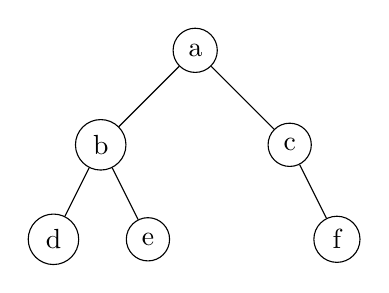
\begin{tikzpicture}[scale=1.2, every node/.style={circle, draw, fill=white}]
\node (a) at (0,0) {a};
\node (b) at (-1,-1) {b};
\node (c) at (1,-1) {c};
\node (d) at (-1.5,-2) {d};
\node (e) at (-0.5,-2) {e};
\node (f) at (1.5,-2) {f};

\draw (a) -- (b);
\draw (a) -- (c);
\draw (b) -- (d);
\draw (b) -- (e);
\draw (c) -- (f);
\end{tikzpicture}
\end{center}

\subsection{Ejemplos y contraejemplos}

\begin{exampleblock}{¿Cuáles de los siguientes grafos son árboles?}
\begin{center}
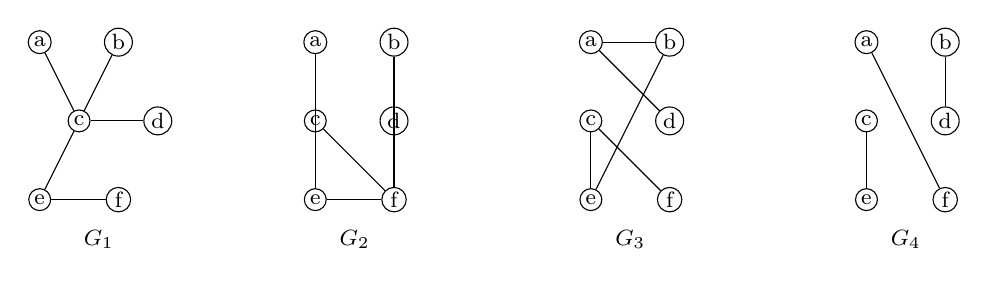
\begin{tikzpicture}[scale=1, every node/.style={circle, draw, inner sep=1pt, font=\footnotesize}]
% G1
\node (a1) at (0,2) {a};
\node (b1) at (1,2) {b};
\node (c1) at (0.5,1) {c};
\node (d1) at (1.5,1) {d};
\node (e1) at (0,0) {e};
\node (f1) at (1,0) {f};
\draw (a1) -- (c1);
\draw (b1) -- (c1);
\draw (c1) -- (d1);
\draw (c1) -- (e1);
\draw (e1) -- (f1);
\node[draw=none, fill=none] at (0.75,-0.5) {$G_1$};

% G2
\begin{scope}[xshift=3.5cm]
\node (a2) at (0,2) {a};
\node (b2) at (1,2) {b};
\node (c2) at (0,1) {c};
\node (d2) at (1,1) {d};
\node (e2) at (0,0) {e};
\node (f2) at (1,0) {f};
\draw (a2) -- (e2);
\draw (b2) -- (f2);
\draw (c2) -- (f2);
\draw (e2) -- (f2);
\node[draw=none, fill=none] at (0.5,-0.5) {$G_2$};
\end{scope}

% G3
\begin{scope}[xshift=7cm]
\node (a3) at (0,2) {a};
\node (b3) at (1,2) {b};
\node (c3) at (0,1) {c};
\node (d3) at (1,1) {d};
\node (e3) at (0,0) {e};
\node (f3) at (1,0) {f};
\draw (a3) -- (b3);
\draw (a3) -- (d3);
\draw (c3) -- (e3);
\draw (c3) -- (f3);
\draw (e3) -- (b3);
\node[draw=none, fill=none] at (0.5,-0.5) {$G_3$};
\end{scope}

% G4
\begin{scope}[xshift=10.5cm]
\node (a4) at (0,2) {a};
\node (b4) at (1,2) {b};
\node (c4) at (0,1) {c};
\node (d4) at (1,1) {d};
\node (e4) at (0,0) {e};
\node (f4) at (1,0) {f};
\draw (a4) -- (f4);
\draw (b4) -- (d4);
\draw (c4) -- (e4);
\node[draw=none, fill=none] at (0.5,-0.5) {$G_4$};
\end{scope}
\end{tikzpicture}
\end{center}
\end{exampleblock}

\subsection{Aplicaciones de los árboles}

Los árboles son útiles en múltiples contextos, como se muestra a continuación:

\begin{itemize}
  \item \textbf{Búsqueda y ordenamiento:} Los \emph{árboles binarios de búsqueda} (BST) permiten organizar datos de forma que cada nodo tiene a lo sumo dos hijos. El hijo izquierdo contiene valores menores y el derecho, mayores. Esto permite búsquedas, inserciones y eliminaciones en tiempo promedio \( O(\log n) \), si el árbol está balanceado. Son usados en estructuras de datos como sets, maps y en bases de datos.

  \item \textbf{Compresión de datos:} El algoritmo de \emph{Huffman} construye un árbol binario donde cada hoja representa un símbolo, y la ruta desde la raíz define su código binario. Los símbolos más frecuentes tienen códigos más cortos, minimizando la longitud promedio del mensaje. Estos árboles son fundamentales en formatos como JPEG, MP3 y ZIP.


  \item \textbf{Modelado de juegos:} En teoría de juegos, los árboles modelan todos los posibles estados y jugadas. Cada nodo representa un estado, y las ramas, movimientos. Son esenciales en juegos como ajedrez o tic-tac-toe. Algoritmos como \emph{minimax} y \emph{poda alfa-beta} operan sobre estos árboles para decidir jugadas óptimas.

\begin{center}
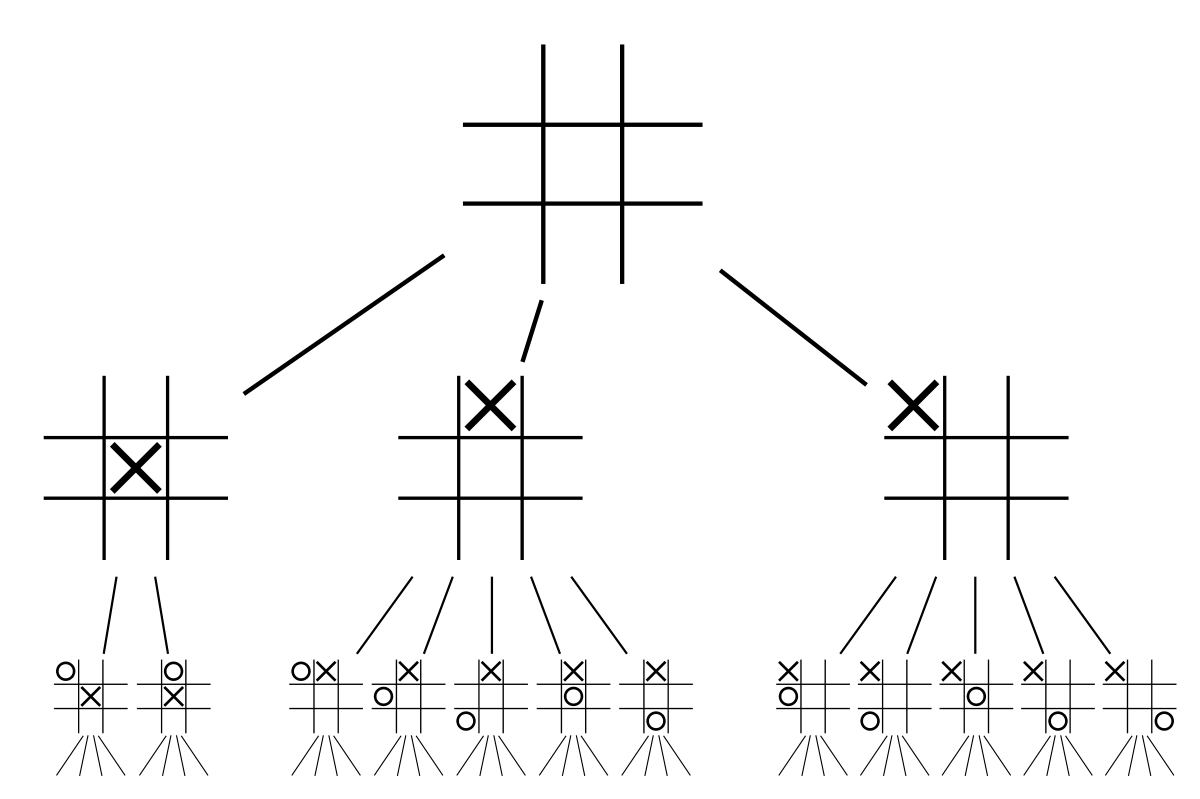
\includegraphics[width=0.45\textwidth]{Figures/tictactoetree.png}
\end{center}
\begin{center}\small\textit{Figura: Árbol de decisiones del juego Tic-Tac-Toe.}\end{center}

  \item \textbf{Estructuración de información:} Formatos como \emph{XML} y \emph{JSON} representan información anidada de forma jerárquica usando árboles. Cada nodo es una etiqueta o clave, y sus hijos representan contenido anidado. Esto facilita la consulta (e.g. con XPath), la transformación, y la validación de documentos.

  \item \textbf{Representación de decisiones:} En \emph{machine learning}, los árboles de decisión modelan decisiones mediante tests secuenciales sobre los datos. Cada nodo representa una pregunta; las ramas, respuestas posibles; y las hojas, una predicción. Son la base de modelos como CART, Random Forest y XGBoost, destacándose por su interpretabilidad.
\end{itemize}

% \subsubsection*{Árbol binario de búsqueda (BST)}

% \begin{center}
% \begin{tikzpicture}[level distance=1.2cm,
%   level 1/.style={sibling distance=2.8cm},
%   level 2/.style={sibling distance=1.4cm},
%   every node/.style={circle, draw}]
% \node {8}
%   child {node {3}
%     child {node {1}}
%     child {node {6}}}
%   child {node {10}
%     child[missing]
%     child {node {14}}};
% \end{tikzpicture}
% \end{center}

% \subsubsection*{Códigos de Huffman}

% \begin{center}
% \begin{tikzpicture}[sibling distance=8mm,
%   level distance=10mm,
%   every node/.style = {circle, draw, font=\tiny}]
% \node { }
%   child {node {a}}
%   child {node { }
%     child {node {b}}
%     child {node { }
%       child {node {c}}
%       child {node {d}}}};
% \end{tikzpicture}
% \end{center}

% \textbf{Ventaja:} el código es \emph{prefix-free} (ningún código es prefijo de otro), lo que permite decodificar sin ambigüedad.



\begin{center}
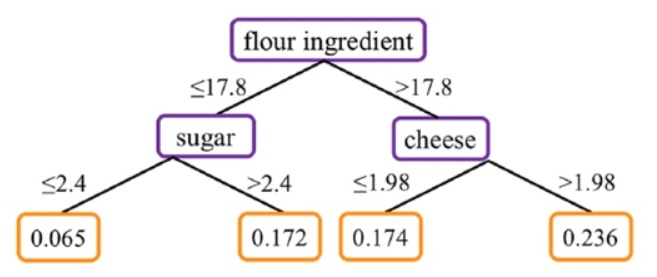
\includegraphics[width=0.5\textwidth]{Figures/tree_food_crop}
\end{center}
\begin{center}\small\textit{Figura: Árbol de regresión con tres predictores (harina, azúcar y queso), utilizado para clasificar países según su consumo y predecir prevalencia de obesidad en cuatro grupos distintos.
 Fuente: Dunstan, J., et al. (2020). Predicting nationwide obesity from food sales using machine learning.}\end{center}



\subsection{Caracterizaciones alternativas}


A primera vista, la definición de árbol puede parecer un tanto arbitraria: un grafo que es \emph{conexo} y \emph{acíclico}. Pero, ¿por qué esas dos condiciones en particular? Para responder esta pregunta, es útil considerar qué implican esas propiedades en términos de la estructura del grafo.

\textbf{Conexión} significa que hay un camino entre cada par de nodos. Es decir, el grafo debe tener suficientes aristas para mantener todos los vértices conectados en una sola componente. Por otro lado, \textbf{no tener ciclos} nos obliga a restringir el número de conexiones: no puede haber más aristas que las necesarias, porque cualquier exceso podría cerrar un ciclo.

Los árboles, entonces, se sitúan exactamente en el \emph{punto de equilibrio} entre tener suficientes aristas para ser conexos, pero no tantas como para crear ciclos. Este balance permite que muchas propiedades estructurales equivalentes emerjan, como veremos en el siguiente teorema.


\begin{exampleblock}{Teorema}
Sea $G=(V,E)$ un grafo no dirigido. Las siguientes propiedades son equivalentes:
\begin{enumerate}
  \item $G$ es un árbol;
  \item $G$ contiene un único camino simple entre cada par de nodos distintos;
  \item $G$ es conexo y $|E| = |V| - 1$.
\end{enumerate}
\end{exampleblock}

\subsubsection*{Demostraciones}

\paragraph{1 $\Rightarrow$ 2:} Sea $u$ y $v$ vértices distintos de $G$. Como $G$ es un árbol, es conexo y por lo tanto existe un camino simple que los conecta. 

Supongamos que hay dos caminos simples distintos entre $u$ y $v$: $C_1$ y $C_2$. Esto implicaría la existencia de un ciclo simple en $G$, contradiciendo la hipótesis.

Si divergen antes de finalizar, los caminos generan un ciclo entre el primer punto de divergencia $x$ y el de reencuentro $y$:
\begin{center}
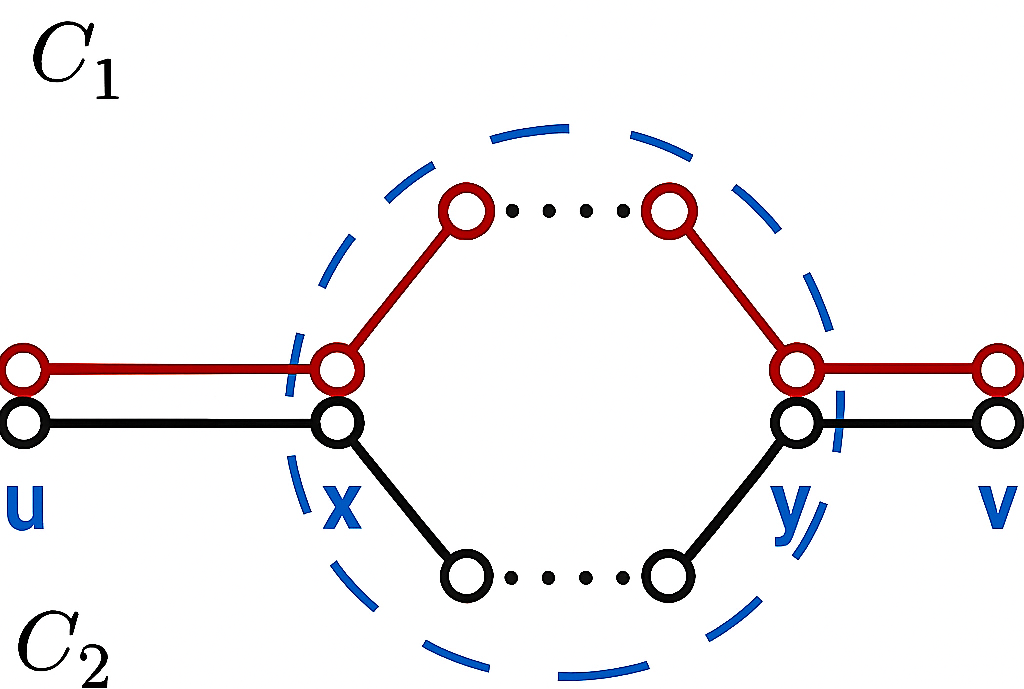
\includegraphics[width=0.35\textwidth]{Figures/ciclo.png}
\end{center}

\paragraph{2 $\Rightarrow$ 1:} Por hipótesis, existe un único camino simple entre cada par de nodos. Esto implica que $G$ es conexo. Supongamos ahora que $G$ contiene un ciclo simple. Entonces, entre dos nodos de ese ciclo hay más de un camino simple, contradiciendo la unicidad. \hfill $\square$

\paragraph{1 $\Rightarrow$ 3:} Demostración por inducción fuerte sobre $|E|$.

\textit{HI:} Para todo árbol con $|E| \leq d$, se cumple $|E| = |V| - 1$.

Consideremos un árbol cualquiera $G$ con $|E| = d + 1$.  Sea  $G\setminus{a}$ el grafo que se forma quitando de $G$ la arista $a$ tal que el árbol no es conexo,  i.e.,  $G\setminus{a}= G_1 \cup G_2$,  donde $G_1$ y $G_2$ son árboles con no más de $d$ aristas.
Por la caracterización 2, toda arista es esencial: si se elimina, el grafo se desconecta.

Aplicamos a $G_1$ y $G_2$ la HI: $|E(G_i)|=|V_i|-1$ y sumando obtenemos  $|E| - 1 = (|V_1| - 1) + (|V_2| - 1) = |V| - 2$, por lo tanto $|E| = |V| - 1$.
\hfill $\square$

\paragraph{3 $\Rightarrow$ 1:} Supongamos que $G$ es conexo y $|E| = |V| - 1$, pero que contiene un ciclo. Eliminamos una arista del ciclo. El nuevo grafo $G'$ sigue siendo conexo pero ahora tiene $|E| < |V| - 1$,  lo cual es imposible.

De hecho, \textbf{todo grafo conexo debe tener al menos $|V| - 1$ aristas}, pues de lo contrario no es posible conectar todos los vértices.
\hfill $\square$


\subsection{Árboles con raíz}

En muchas aplicaciones es útil distinguir un nodo particular como la \textbf{raíz} del árbol. A menudo, en los \textbf{árboles con raíz} se orientan las aristas para que apunten \emph{lejos} de la raíz.

\begin{center}
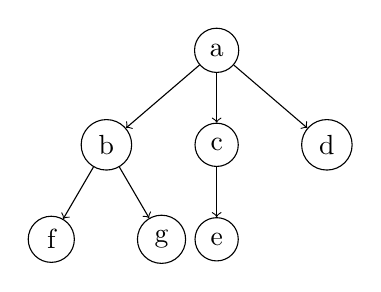
\begin{tikzpicture}[->, every node/.style={circle, draw}, level distance=1.2cm, sibling distance=1.4cm]
\node (a) {a}
  child {node (b) {b}
    child {node {f}}
    child {node {g}}}
  child {node (c) {c}
    child {node {e}}}
  child {node {d}};
\end{tikzpicture}
\end{center}

\subsection*{Terminología básica}
Sea $T$ un árbol con raíz $v$:
\begin{itemize}
  \item El \textbf{padre} de un nodo $u \neq v$ es el vértice desde el cual se llega a $u$ por una arista dirigida. A su vez, $u$ es un \textbf{hijo} de ese vértice.
  \item Dos nodos son \textbf{hermanos} si tienen el mismo padre.
  \item Los \textbf{ancestros} de $u$ son los nodos en el camino desde $u$ hacia la raíz. Sus \textbf{descendientes} son los nodos que tienen a $u$ como ancestro.
  \item Una \textbf{hoja} es un nodo sin hijos; los demás se llaman \textbf{internos}.
  \item La \textbf{altura} del árbol es la longitud del camino más largo desde la raíz hacia cualquier hoja.
\end{itemize}

\subsection{Árboles $m$-arios}

A veces interesa restringir la cantidad de hijos que puede tener un nodo.

\begin{exampleblock}{Definición}
Un árbol con raíz es \textbf{$m$-ario} ($m \geq 1$) si cada nodo interno tiene a lo más $m$ hijos. Es \textbf{completo} si todos los nodos internos tienen exactamente $m$ hijos.
\end{exampleblock}

\begin{center}
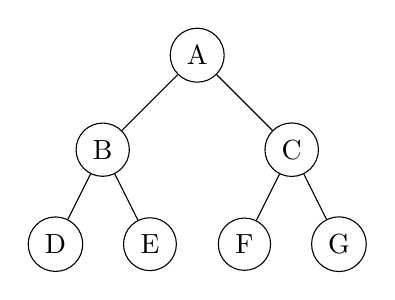
\begin{tikzpicture}[level distance=1.2cm,
  level 1/.style={sibling distance=2.4cm},
  level 2/.style={sibling distance=1.2cm},
  every node/.style={circle, draw}]
\node {A}
  child {node {B}
    child {node {D}}
    child {node {E}}}
  child {node {C}
    child {node {F}}
    child {node {G}}};
\end{tikzpicture}
\end{center}

\subsection*{Propiedades fundamentales}
\begin{exampleblock}{Teorema}
\begin{itemize}
  \item Si $T$ es un árbol $m$-ario de altura $h$, entonces tiene a lo sumo $m^h$ hojas.
  \item Si $T$ es un árbol $m$-ario completo con $i$ nodos internos, entonces tiene $m \cdot i + 1$ nodos en total.
\end{itemize}
\end{exampleblock}

\subsection*{Ejercicios}

\newboxquestion{P1} Sea $G$ un grafo no dirigido. Probar que $G$ es un árbol si y sólo si $G$ es conexo, pero sacarle cualquier arista lo vuelve disconexo.
\begin{proof}
\leavevmode

\paragraph{\( \Rightarrow \)}
Asuma que $G = (V, E)$ es un árbol. Queremos probar que quitar cualquier arista lo desconecta.

\begin{itemize}
  \item Como $G$ es un árbol, es conexo por definición.
  \item Supongamos por contradicción que existe una arista $e \in E$ tal que el grafo $G' = (V, E \setminus \{e\})$ sigue siendo conexo.
  \item Entonces $G'$ sería un grafo conexo y sin ciclos (porque $G$ no tenía ciclos y quitar una arista no puede crear uno), es decir, también un árbol.
  \item Pero entonces: $|E| = |V| - 1$ y $|E \setminus \{e\}| = |V| - 2$, lo que contradice la caracterización 3.
\end{itemize}

\paragraph{ \( \Leftarrow \)}
Asuma que $G = (V, E)$ es conexo, y que quitar cualquier arista lo desconecta. Queremos probar que $G$ no tiene ciclos simples.

\begin{itemize}
  \item Supongamos por contradicción que $G$ contiene un ciclo simple $C$.
  \item Entonces podemos quitar una arista de $C$ y el grafo seguiría siendo conexo, ya que los vértices del ciclo seguirían conectados por el resto del ciclo.
  \item Esto contradice la hipótesis de que quitar cualquier arista desconecta $G$.
\end{itemize}

\end{proof}

\newboxquestion{P2} Demuestra que cualquier árbol es un grafo bipartito.


\begin{proof}
Como $T$ es un árbol, no contiene ciclos. Vamos a demostrar que $T$ es bipartito, es decir, que su conjunto de vértices $V$ se puede dividir en dos subconjuntos disjuntos $V_1$ y $V_2$ tal que ninguna arista conecta dos vértices dentro del mismo subconjunto.

Elegimos un vértice arbitrario $v \in V$ y definimos $V_1$ como el conjunto de vértices a distancia par de $v$ y $V_2$ como aquellos a distancia impar.

Como $T$ es un grafo sin ciclos, la distancia entre dos vértices cualesquiera está bien definida y única. Toda arista conecta dos vértices cuyas distancias respecto a $v$ difieren en exactamente 1 (ya que no hay ciclos), por lo que nunca une dos vértices ambos en $V_1$ ni ambos en $V_2$.

Por lo tanto, $T$ es bipartito.
\end{proof}

\newboxquestion{P3}  Ecuentre el número de árboles no isomórficos con 5 vértices
